\section{INTRODUCTION}
Recently, aerial robots have attracted a lot of attention and have been studied actively due to their high mobility in three-dimensional environments\cite{Kumar2012}. While there are many application of aerial robots, such as surveillance\cite{surveillance}, rescue\cite{rescue}, object manipulation and transportation by aerial robots has become an active area of research\cite{lindsey2012}\cite{Mellinger2011}\cite{ZhaoICRA2017}\cite{Bernard2009}\cite{Hugh2012}. However, there are still some problems to solve about aerial object transportation. In particular, the endurance of aerial robots is a significant problem. To make the endurance longer, putting bigger batteries can be considered as a way, but the endurance does not scale linearly with the batteries capacity due to their large weight. Moreover, large weight causes instability of flight. Therefore, it is not easy to make the endurance longer, so we must change the point of view. 
\par
To improve the efficiency of aerial object transportation within the limited endurance, we focus on a way that aerial robot transports multiple objects at the same time. However, it is difficult for conventional aerial robots to transport multiple objects because multiple grippers are necessary to grasp multiple objects, but when the number of objects the aerial robot grasps changes, the center of gravity(CoG) position of the aerial robot changes, resulting that the flight control becomes unstable. Therefore, to achieve this purpose, we focus on multirotor with two-dimensional multilinks\cite{Zhao2016} which has the ability to modify the CoG position actively. When picking up an object, the multirotor with multilinks can keep the flight control stable by the aerial transformation by which the CoG position can be modified. 
\par
The main purpose of this paper is to achieve the multiple objects transportation by the multirotor with multilinks, along with the configuration of hardware and software system. Sec. II describes the general approach for the multiple objects transportation. Sec. III clarifies the model of the transformable aerial robot and flight control for aerial transformation.  Sec. IV explains how to find the optimal form of the multirotor with multilinks based on the flight stability. In Sec. V, the hardware and software system of the multirotor with multilinks is proposed. Finally, we present experimental results in Sec. VI to demonstrate the feasibility of the multiple object transportation by the multirotor with multilinks. 
\begin{figure}[t]
  \begin{center}
    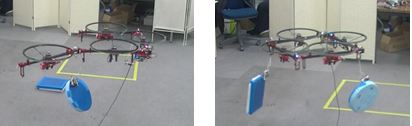
\includegraphics[width=1.0\columnwidth]{figs/object_transportation.png}
  \end{center}
  \caption{The multiple object transportation achieved by the transformable aerial robot. Left: the aerial robot grasps one object. Right: the aerial robot grasps two objects.}
  \label{figure:system}
\end{figure}
